\subsection{UC27 - Logout}\label{usecase:27}
\begin{figure}[H]
\centering
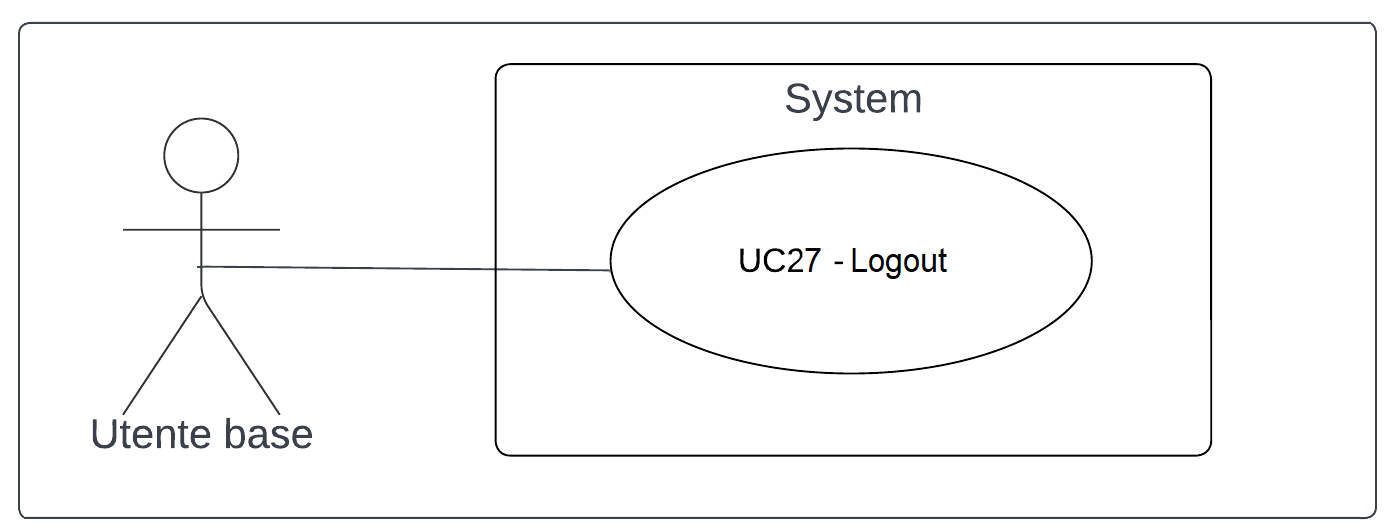
\includegraphics[width=0.75\linewidth]{ucd/UCD27.png}
\caption{Logout}
\end{figure}
\textbf{Attori}:
\begin{itemize}
    \item Utente autenticato.
\end{itemize}
\textbf{Precondizioni}:
\begin{itemize}
    \item L'utente è connesso nel sistema.
\end{itemize}
\textbf{Postcondizioni}:
\begin{itemize}
    \item L'utente è stato disconnesso dal sistema e non può accedere a funzionalità riservate agli utenti autenticati fino a quando non esegue nuovamente l'accesso.
\end{itemize}
\textbf{Scenario principale}:
\begin{enumerate}
    \item L'utente seleziona l'opzione di logout dal sistema;
    \item Il sistema conferma la richiesta di logout;
    \item Il sistema termina la sessione dell'utente e reindirizza l'utente alla pagina di accesso.
\end{enumerate}

\newpage